\documentclass[a4paper,12pt,titlepage]{article}
\usepackage{palatino}
\usepackage{graphicx}
\usepackage{float}
\usepackage{amsmath}
\usepackage{caption}
\usepackage{subcaption}
\usepackage[margin=1.5cm,includefoot]{geometry}
\usepackage[utf8]{inputenc}
\usepackage{hyperref}
\usepackage{url}
\usepackage{listings}
\usepackage{xcolor}
\definecolor{bluekeywords}{rgb}{0.13,0.13,1}
\definecolor{greencomments}{rgb}{0,0.5,0}
\definecolor{redstrings}{rgb}{0.9,0,0}


\renewcommand*{\familydefault}{\sfdefault}
\usepackage[portuguese]{babel}

\usepackage{listings}
\lstset{language=[Sharp]C,
	showspaces=false,
	showtabs=false,
	breaklines=true,
	showstringspaces=false,
	breakatwhitespace=true,
	escapeinside={(*@}{@*)},
	commentstyle=\color{greencomments},
	keywordstyle=\color{bluekeywords}\bfseries,
	stringstyle=\color{redstrings},
	basicstyle=\ttfamily
}

%\lstdefinestyle{sharpc}{language=[Sharp]C, frame = lrtb, rulecolor=\color{blue!80!black}}




\title{\textbf{ \Huge{Integração entre PSoC e Smartphone}}\\}

\author{Victor São Paulo Ruela\\
	Universidade Federal de Minas Gerais}

\date{\today}

%\renewcommand*\contentsname{Sumário}


\begin{document}


\maketitle

\tableofcontents
\newpage

\section{Introdução}
	O projeto consiste na integração de dados entre um system-on-ship (PSoC) e um aplicativo Android, utilizando para isso um Web Service na plataforma .NET.
	Através do aplicativo, o usuário consegue visualizar a temperatura do PSoC pressionando um botão. Também foi implementado um cliente Web para consumir o Web Service. Este cliente possui um botão para requisitar a leitura da temperatura do PSoC e a partir dessas leituras, constrói uma tabela contendo todos os valores lidos. Portanto, a seguinte arquitetura de integração foi implementada:
	
	\begin{figure}[h!]
		\centering
		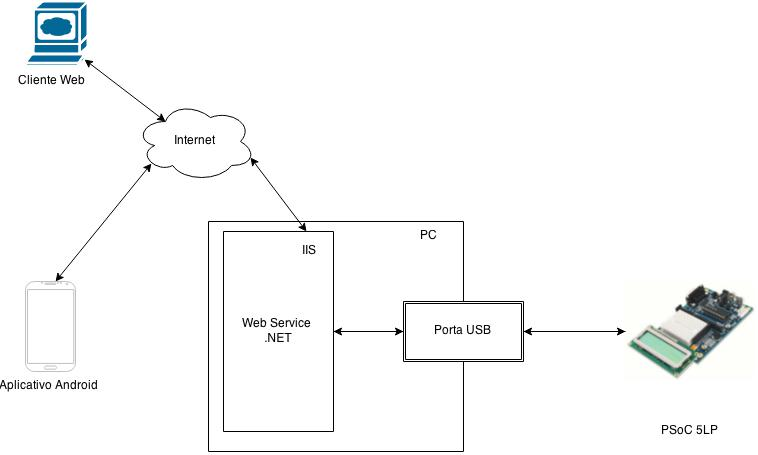
\includegraphics[width=0.7\linewidth]{arquitetura}
		\caption{Arquitetura da integração}
		\label{fig:diagrama}
	\end{figure}
	  
\section{Implementação}
	\subsection{Aplicação do PSoC}
		A aplicação foi feita no PSoC Creator. A criação de uma aplicação para o PSoC é feita através de diagrama de blocos e em C. Inicialmente, colocamos as instâncias dos componentes que serão utilizados em uma página do arquivo \textbf{TopDesig.cysch}, que é o padrão de qualquer projeto no PSoC Creator. Depois precisamos inicializar e interligar os diversos componentes através de suas APIs, em linguagem C. Para este projeto, foi foram necessários os componentes \textbf{DieTemp} e \textbf{USBUART}. O primeiro permite a leitura da temperatura do PSoC enquanto o segundo habilita o uso da porta USB da placa. Ambos foram usados com a configuração padrão.
			\begin{figure}[h!]
				\centering
				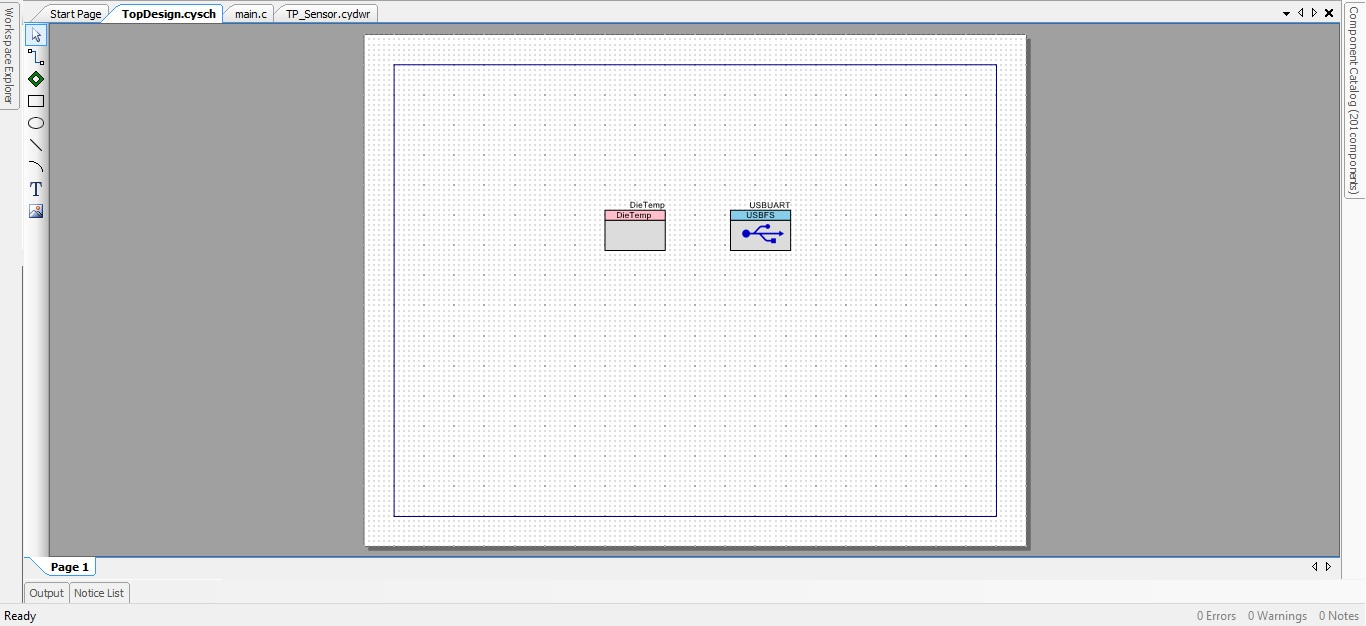
\includegraphics[width=1\linewidth]{psoc1}
				\caption{Diagram de blocos no PSoC}
				\label{fig:psoc1}
			\end{figure}
		
		O código em C utiliza as funções da API de cada componente. A lógica de funcionamento da aplicação é bem simples:
			\begin{enumerate}
				\item Inicializar o componente \textbf{USBUART}
				\item Aguardar enumeração da porta USB
				\item Aguardar mensagem de requisiçao de leitura
				\item Obter temperatura através do bloco \textbf{DieTemp}
				\item Enviar para a porta USB				  
			\end{enumerate}
		O PSoC fica em um loop infinito aguardando novas mensagens de requisição de leitura. O bloco USBUART funciona como uma porta serial COM, facilitando a leitura e escrita de dados pela aplicação \textbf{.NET} do Web Service. 
		
			 
	\subsection{Web Service}
		O Web Service está implementado na platforma .NET versão 4.0, usando a linguagem C\#. Ele será publicado em um servidor web local através do \textbf{IIS - Internet Information Services}. Foi necessário realizar uma configuração do roteador: redirecionamento da porta 80 ao endereço de IP local da máquina conectada ao PSoC, para tornar o Web Service visível a todos os computadores e dispositivos conectados à rede. 
		A publicação de Web Service foi facilitada com o uso do \textbf{MS Visual Studio 2012}, o qual possui uma ferramenta muito útil para a publicação de aplicações Web. Isso reduziu bastante o tempo necessário para desenvolver a aplicação, uma vez que não foram encontrados muitos problemas relacionados à configuração do IIS. O Web Service foi configurado para funcionar com o protocolo SOAP e os métodos  GET e POST do HTTP. 
		
		\subsubsection{Estrutura da aplicação}
			Decidi por implementar o Web Service usando ASMX, porque ele é mais simples e fácil de configurar, e atendia a todos os requisitos do projeto: uso do HTTP(SOAP) e do IIS. O WCF também poderia ser usado, mas é uma ferramenta mais avançada e poderosa. Como a aplicação desenvolvida é simples, seu uso se mostrou desnecessário.   
			O Web Service fornece dois serviços:
			\paragraph{ReadPSoC}
				Serviço responsável pela comunicação com o PSoC através da porta USB, consumido principalmente pelo aplicativo Android. Inicialmente, ele obtém uma lista de valores de temperatura através da variável Session, que contém os dados de sessão para um determinado usuário. Feito isso, começa a troca de dados propriamente dita:
				\begin{enumerate}
					\item Criação do objeto SerialPort:
								\begin{lstlisting}	
SerialPort s = new SerialPort("COM3", 9600);
								\end{lstlisting}
						  O parâmetro COM3 é o número da porta COM e 9600 é a baudrate da porta, definida na configuração do bloco USBUART.
					\item Abertura da porta serial:
								\begin{lstlisting}	
s.Open();
								\end{lstlisting}
					\item Escrita e leitura na porta serial:
								\begin{lstlisting}	
s.WriteLine("OK");
line = s.ReadLine();								
								\end{lstlisting}
							O dado lido também é adicionado à lista descrita acima, para ficar disponível ao usuário da aplicação Web.
					\item Fechamento da porta serial:
								\begin{lstlisting}	
s.Close();
								\end{lstlisting}
																  
				\end{enumerate}
			As funções acima fazem parte da biblioteca \textbf{System.IO.Ports} do .NET.
			O código possui tratamento de exceções para evitar que a leitura falhe e comprometa a integração do sistema. A principal exceção gerada ocorre quando tentamos ler com o PSoC desconectado do computador. Nesse caso, o Web Service envia a mensagem "Error opening port", indicando a falha. 
			O serviço retorna uma string, contendo a temperatura lida e uma \textit{time stamp} indicando o momento em que a leitura foi feita.
		
			\paragraph{getReadings}
				Serviço usado pela aplicação Web, que será explicada com mais detalhes à frente. Ela retorna uma lista de strings contendo as temperaturas lidas salvas na variável Session do usuário. 
				
		  Ambos os servicos são definidos como \textbf{[WebMethod(EnableSession=true)]}. Esse parâmetro permite salvar e recuperar valores do usuário que está acessando página Web. 
	
	\subsection{Aplicativo Android}	
			O aplicativo foi implementado em Java, usando as bibliotecas do pacote Android SDK tools. A comunicação com o Web Service é feita com o protocolo SOAP.
			
			\subsubsection{Interface gráfica}
				A interface gráfica é bem simples, e consiste de um \textbf{EditText} \cite{EditText} para o usuário digitar o IP, um \textbf{TextView} \cite{TextView} para exibir a temperatura e um \textbf{Button} \cite{Button} para requisitar um serviço do Web Service. A interface gráfica será exibida na seção dos resultados nas figuras \ref{fig:nexus4} e \ref{fig:emulador}.
				
			\subsubsection{Estrutura da aplicação}
			O aplicativo foi implementado usando duas classes: \textbf{MainActivity} e \textbf{XMLResponseHandler}. 
			\paragraph{MainActivity} Consiste na atividade principal (thread primária). É responsável por atualizar o IP digitado e realizar as ações necessárias quando o botão é pressionado. Quando isso ocorre, o seguinte código é executado:
			\begin{lstlisting}
public void onClick(View v) {
			
	URL = "http://" + editText.getText() + "/WS_TP/Service1.asmx/ReadPSoC";
	new HttpGetTask().execute();
			
}
			\end{lstlisting}		
			
			Esse método cria uma thread secundária que inicia a comunicação com o Web Service. Esta é considerada uma boa prática em aplicativos Android, pois evita que a interface gráfica fique congelada enquanto a comunicação está sendo processada. A thread executa o seguinte código depois de criada:
			\begin{lstlisting}
private class HttpGetTask extends AsyncTask<Void, Void, String> {
		
	AndroidHttpClient mClient = AndroidHttpClient.newInstance("");
	
	@Override
	protected String doInBackground(Void... params) {
		HttpGet request = new HttpGet(URL);
		XMLResponseHandler responseHandler = new XMLResponseHandler();
		try {
			return mClient.execute(request, responseHandler);
		} catch (ClientProtocolException e) {
			e.printStackTrace();
		} catch (IOException e) {
			e.printStackTrace();
		}
	return null;
	}

			\end{lstlisting}
			A thread é uma extensão da classe \textbf{AsyncTask} \cite{asynctask} e consegue comunicar-se com o Web Service criando, inicialmente, uma instância da classe \textbf{AndroidHttpClient} \cite{httpclient}, que é uma implementação de um cliente HTTP configurado para o Android. Feito isso, são criadas uma instância da classe \textbf{HttpGet}, que implementa o método HTTPGET definido no protocolo HTTP, e da \textbf{XMLResponseHandler} que é responsável por processar a mensagem XML recebida. Finalmente, executamos o cliente HTTP passando os objetos anteriores como parâmetros.
			
			\paragraph{XMLResponseHandler} Classe utilizada para processar a mensagem recebida em XML. Ela utiliza a API \textbf{XMLPULL V1} para processar a XML e obter a informação desejada, no caso a temperatura do PSoC. Seu funcionamento é simples e direto, e está bem descrito em:  \url{http://www.xmlpull.org/}. 
			A informação extraída é salva na variável associada ao \textbf{TextView} que então atualiza a temperatura exibida na UI.
				
	
	\subsection{Cliente Web}
		O cliente Web foi implementado usando Web Forms ASP.NET. A página foi desenvolvida em HTML e contém uma breve descrição de sua funcionalidade, um botão para requisitar a leitura do PSoC e uma tabela mostrando os valores recentemente lidos pelo usuário. Ao clicar no botão, o seguinte script em C\# é executado:
			\begin{lstlisting}	
 protected void btnRead_Click(object sender, EventArgs e)
 {
	 // Criar instancia do objeto ReadPSoCService
	 ReadPSoCService.Service1SoapClient client =
			 new ReadPSoCService.Service1SoapClient();
 
	 // Realiza leitura do PSoC
	 string result = client.ReadPSoC();
	 // Exibe o resultado na pagina
	 lblResult.Text = result;
 
	 // Associa a variavel com os valores da tabela a lista retornada pelo servico
	 gvReadings.DataSource = client.getReadings();
	 gvReadings.DataBind();
	
	 // Altera titulo da tabela 
	 gvReadings.HeaderRow.Cells[0].Text = "Recent Temperature Readings";
 }
 
 
	 		\end{lstlisting}
			Inicialmente, precisamos adicionar ao projeto no MS Visual Studio uma referência ao serviço fornecido pelo Web Service. Feito isso, criamos uma instância de um objeto representando o serviço acima. Logo, podemos acessar ambos os serviços definidos anteriormente (\textbf{ReadPSoC} e \textbf{getReadings}). \textbf{ReadPOsC} é usado para fazer a leitura do PSoC quando clica-se no botão e \textbf{getReadings} é necessária para montar a tabela com os valores lidos, pois ela acessa a variável contendo os dados de sessão do ususário. 
			 
		
\section{Resultados}
	Todos os testes foram realizados com os dispositivos conectados à rede local.  
	\subsection{Cliente Web}
	O cliente Web foi testado em diversos computadores e seu funcionamento foi como o esperado em todos os casos. A página web foi acessada de um computador com sistema operacional Windows, outro com Mac OS X e de smartphones, funcionando corretamente em todos. 
	
	\begin{figure}[h!]
		\centering
		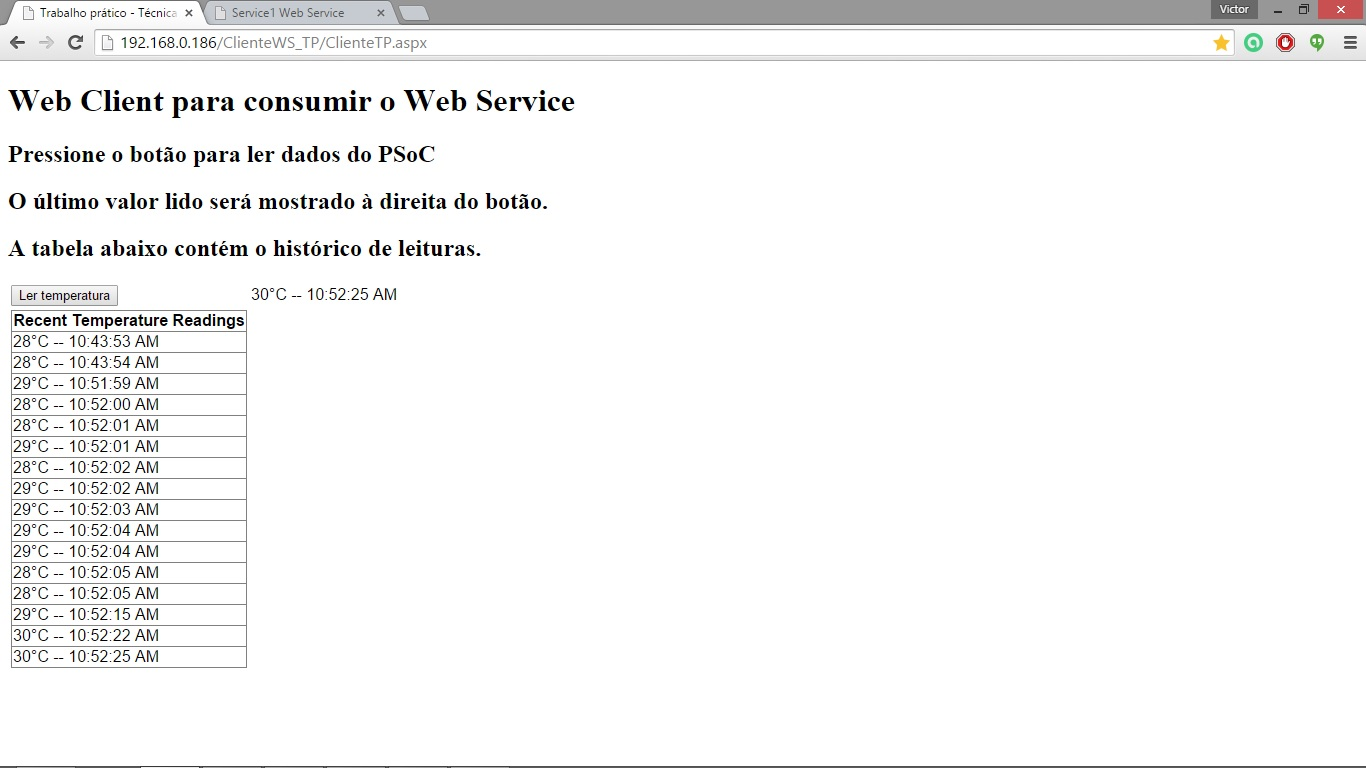
\includegraphics[width=0.5\linewidth]{clienteweb}
		\caption{Funcionamento do cliente Web}
		\label{fig:clienteweb}
	\end{figure}
	
	\subsection{Aplicativo Android}
	O aplicativo foi testado no emulador de dispositivos Android e em um Nexus 4. Ambos funcionaram perfeitamente.
	
		\begin{figure}[h!]
			\centering
			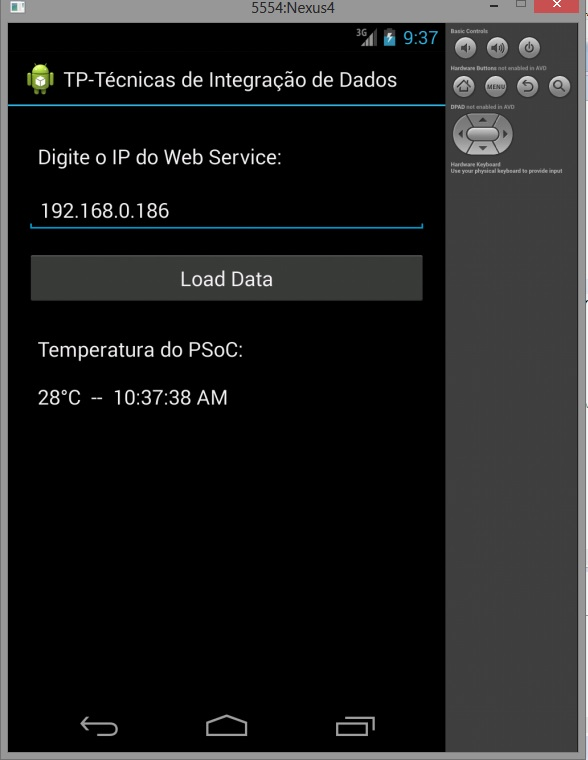
\includegraphics[width=0.3\linewidth]{appemulador}
			\caption{Screenshot do emulador de Dispositivos Android}
			\label{fig:emulador}
		\end{figure}
		
		\begin{figure}[h!]
			\centering
			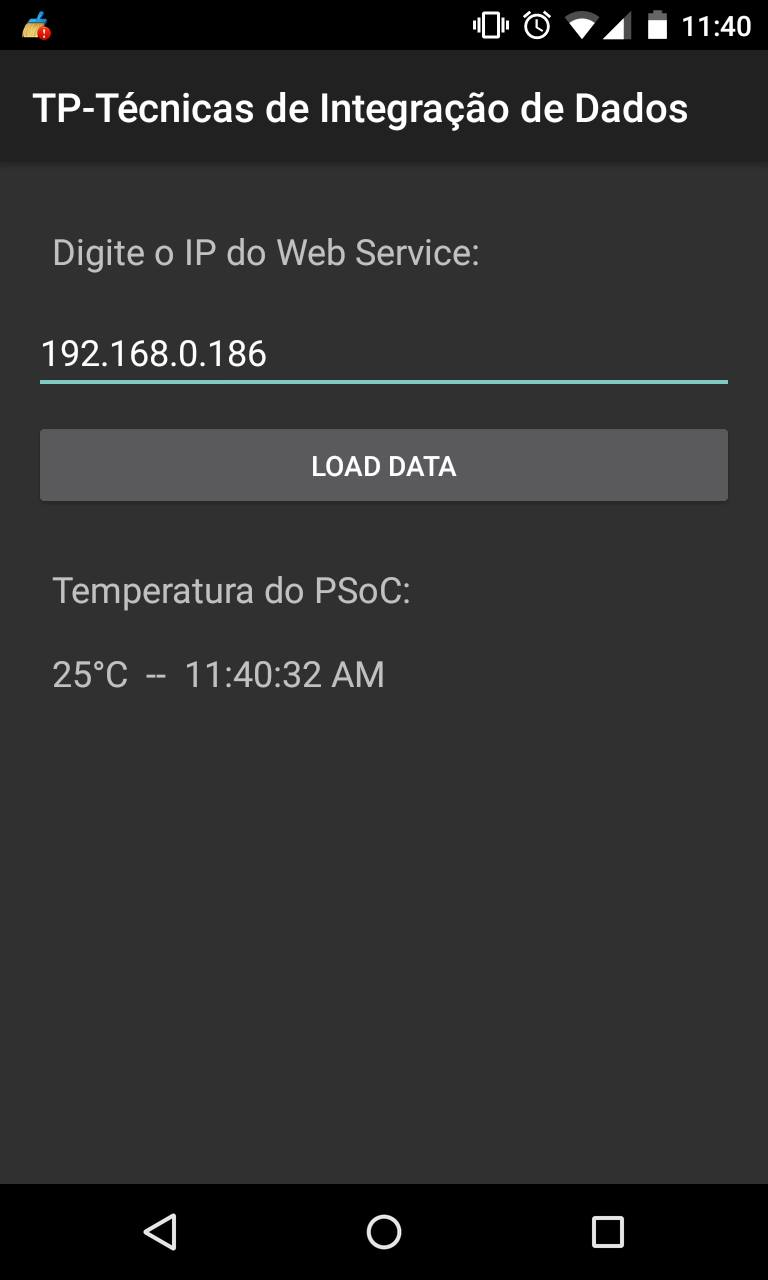
\includegraphics[width=0.3\linewidth]{appnexus}
			\caption{Screenshot de um Nexus 4}
			\label{fig:nexus4}
		\end{figure}
\section{Dificuldades encontradas}
	A implementação do trabalho ocorreu sem muitos problemas, mas algumas dificuldades foram encontradas e serão descritas a seguir.
	\paragraph{Driver USB do PSoC} Este sem dúvidas foi o maior problema encontrado. Ao compilarmos e gravarmos o programa no PSoC, a porta USB para a troca de dados não é automaticamente reconhecida pelo Windows. Portanto, o driver deve ser instalado manualmente, porém ele não é disponibilizado de maneira fácil pela Cypress. Felizmente, no caso do bloco \textbf{USBUART}, o driver é gerado automaticamente na compilação do projeto e fica localizado na pasta "Generated\_Source" do projeto, com o nome \textbf{USBUART\_cdc.inf}. Logo, para resolver este problema é preciso ir no gerenciador de dispositivos do Windows e instalá-lo com o driver citado anteriormente.
	
	\paragraph{Instalação do aplicativo no Smartphone} 
	A instalação do aplicativo no Nexus 4 utilizado nos testes também teve problemas relacionados ao driver. A forma inicialmente utilizada consistia em fazer o upload do aplicativo através do eclipse, com o celular conectado à porta USB. Isso permite debugar o aplicativo rodando no celular. Para isto, devemos baixar e instalar uma aplicação chamada ADB (Android Debug Bridge), a qual contém os drivers necessários. Entretanto, tive diversos problemas com o driver, o qual funcionou algumas vezes mas de uma hora para a outra parou de funcionar, me impossibilitando de carregar o aplicativo no Nexus 4. A solução para este problema foi fazer o upload do arquivo com extensão \textbf{.apk}, que é o aplicativo compilado, para o Dropbox, baixá-lo do Smartphone e por fim instalá-lo manualmente.
	
	\paragraph{Leitura da porta USB}
	Para a leitura/escrita dos dados da porta USB, foi utilizada a biblioteca \textbf{System.IO.Ports} da plataforma .NET. Seu uso é bastante simples, porém ela possui um comportamento que pode ser prejudicial a qualquer aplicação: ao requisitarmos o fechamento da porta, esta demora um intervalo indefinido de tempo para poder ser aberta novamente. Isso faz com que a porta fique bloqueada quando tentamos abrí-la novamente antes de ela ser efetivamente fechada. Esse problema foi observado durante os testes quando requisições eram feitas com um intervalo de tempo muito pequeno entre elas. Se isso ocorre, é preciso reiniciar o computador para conseguir novamente abrir a porta USB. Minha sugestão para evitar esse problema é adicionar uma pequena pausa ao programa, para que haja tempo suficiente para a porta ser efetivamente fechada.
	
	\paragraph{Configuração do Web Service no IIS}	
	A publicação manual do Web Service no IIS não é tão simples e direta. Antes de descobrir a função \textbf{Publish} do Visual Studio 2012, tentei adicionar manualmente o Web Service e ocorriam diversos erros de configuração. Um deles estava relacionado às permissões de acesso à pasta que continha o projeto: é preciso adicionar permissão para que os grupos de usuários \textbf{IUSR} e \textbf{IIS\_IUSRS} possam acessar o conteúdo da pasta. Isso é um requerimento do IIS. Minha sugestão é sempre usar a ferramenta \textbf{Publish}, pois ela já realiza todas essas configurações e reduz bastante o trabalho de realizar esta tarefa. 
	
	 
	
\section{Conclusão}
	Através dos resultados exibidos anteriormente, podemos concluir que a integração entre o PSoC e aplicativo Android/Cliente Web foi realizada com sucesso. Algumas mudanças foram feitas em relação ao projeto original descrito no estudo de viabilidade:
	\begin{itemize}
		\item Utilização do MS Visual Studio 2012 para implementar o Web Service;
		\item O visor LCD não funcionou e foi retirado do projeto;
		\item Desenvolvimento de um cliente Web;
		\item Melhora da interface gráfica do aplicativo.
	\end{itemize}
	
	As mudanças realizadas aumentaram um pouco a complexidade do projeto, porém foram implementadas sem grandes problemas e acrescentaram bastante ao resultado final. Algumas melhorias poderiam ser feitas, e entre elas podemos citar a implementação do Web Service em \textbf{WCF} ao invés de \textbf{ASMX}, de forma a aumentar a robustez da aplicação.
	
	O projeto implementado exemplifica uma forte tendência atual, que é a integração entre Smartphones e diversos tipos de sistemas através de Web Services. A idéia pode ser extendida para aplicações mais complexas e interessantes. Por exemplo, uma aplicação é a monitoração de sinais vitais de pacientes em tempo real, através de um aplicativo consumindo um Web Service. Isso permitiria aos médicos monitorar diversos pacientes de forma mais eficiente e remotamente.     
	
\newpage

\bibliographystyle{plain}
\nocite{*}
\bibliography{biblio_doc}

\end{document}